% Options for packages loaded elsewhere
\PassOptionsToPackage{unicode}{hyperref}
\PassOptionsToPackage{hyphens}{url}
%
\documentclass[
  man]{apa7}
\usepackage{amsmath,amssymb}
\usepackage{lmodern}
\usepackage{iftex}
\ifPDFTeX
  \usepackage[T1]{fontenc}
  \usepackage[utf8]{inputenc}
  \usepackage{textcomp} % provide euro and other symbols
\else % if luatex or xetex
  \usepackage{unicode-math}
  \defaultfontfeatures{Scale=MatchLowercase}
  \defaultfontfeatures[\rmfamily]{Ligatures=TeX,Scale=1}
\fi
% Use upquote if available, for straight quotes in verbatim environments
\IfFileExists{upquote.sty}{\usepackage{upquote}}{}
\IfFileExists{microtype.sty}{% use microtype if available
  \usepackage[]{microtype}
  \UseMicrotypeSet[protrusion]{basicmath} % disable protrusion for tt fonts
}{}
\makeatletter
\@ifundefined{KOMAClassName}{% if non-KOMA class
  \IfFileExists{parskip.sty}{%
    \usepackage{parskip}
  }{% else
    \setlength{\parindent}{0pt}
    \setlength{\parskip}{6pt plus 2pt minus 1pt}}
}{% if KOMA class
  \KOMAoptions{parskip=half}}
\makeatother
\usepackage{xcolor}
\usepackage{graphicx}
\makeatletter
\def\maxwidth{\ifdim\Gin@nat@width>\linewidth\linewidth\else\Gin@nat@width\fi}
\def\maxheight{\ifdim\Gin@nat@height>\textheight\textheight\else\Gin@nat@height\fi}
\makeatother
% Scale images if necessary, so that they will not overflow the page
% margins by default, and it is still possible to overwrite the defaults
% using explicit options in \includegraphics[width, height, ...]{}
\setkeys{Gin}{width=\maxwidth,height=\maxheight,keepaspectratio}
% Set default figure placement to htbp
\makeatletter
\def\fps@figure{htbp}
\makeatother
\setlength{\emergencystretch}{3em} % prevent overfull lines
\providecommand{\tightlist}{%
  \setlength{\itemsep}{0pt}\setlength{\parskip}{0pt}}
\setcounter{secnumdepth}{-\maxdimen} % remove section numbering
% Make \paragraph and \subparagraph free-standing
\ifx\paragraph\undefined\else
  \let\oldparagraph\paragraph
  \renewcommand{\paragraph}[1]{\oldparagraph{#1}\mbox{}}
\fi
\ifx\subparagraph\undefined\else
  \let\oldsubparagraph\subparagraph
  \renewcommand{\subparagraph}[1]{\oldsubparagraph{#1}\mbox{}}
\fi
\newlength{\cslhangindent}
\setlength{\cslhangindent}{1.5em}
\newlength{\csllabelwidth}
\setlength{\csllabelwidth}{3em}
\newlength{\cslentryspacingunit} % times entry-spacing
\setlength{\cslentryspacingunit}{\parskip}
\newenvironment{CSLReferences}[2] % #1 hanging-ident, #2 entry spacing
 {% don't indent paragraphs
  \setlength{\parindent}{0pt}
  % turn on hanging indent if param 1 is 1
  \ifodd #1
  \let\oldpar\par
  \def\par{\hangindent=\cslhangindent\oldpar}
  \fi
  % set entry spacing
  \setlength{\parskip}{#2\cslentryspacingunit}
 }%
 {}
\usepackage{calc}
\newcommand{\CSLBlock}[1]{#1\hfill\break}
\newcommand{\CSLLeftMargin}[1]{\parbox[t]{\csllabelwidth}{#1}}
\newcommand{\CSLRightInline}[1]{\parbox[t]{\linewidth - \csllabelwidth}{#1}\break}
\newcommand{\CSLIndent}[1]{\hspace{\cslhangindent}#1}
\ifLuaTeX
\usepackage[bidi=basic]{babel}
\else
\usepackage[bidi=default]{babel}
\fi
\babelprovide[main,import]{english}
% get rid of language-specific shorthands (see #6817):
\let\LanguageShortHands\languageshorthands
\def\languageshorthands#1{}
% Manuscript styling
\usepackage{upgreek}
\captionsetup{font=singlespacing,justification=justified}

% Table formatting
\usepackage{longtable}
\usepackage{lscape}
% \usepackage[counterclockwise]{rotating}   % Landscape page setup for large tables
\usepackage{multirow}		% Table styling
\usepackage{tabularx}		% Control Column width
\usepackage[flushleft]{threeparttable}	% Allows for three part tables with a specified notes section
\usepackage{threeparttablex}            % Lets threeparttable work with longtable

% Create new environments so endfloat can handle them
% \newenvironment{ltable}
%   {\begin{landscape}\centering\begin{threeparttable}}
%   {\end{threeparttable}\end{landscape}}
\newenvironment{lltable}{\begin{landscape}\centering\begin{ThreePartTable}}{\end{ThreePartTable}\end{landscape}}

% Enables adjusting longtable caption width to table width
% Solution found at http://golatex.de/longtable-mit-caption-so-breit-wie-die-tabelle-t15767.html
\makeatletter
\newcommand\LastLTentrywidth{1em}
\newlength\longtablewidth
\setlength{\longtablewidth}{1in}
\newcommand{\getlongtablewidth}{\begingroup \ifcsname LT@\roman{LT@tables}\endcsname \global\longtablewidth=0pt \renewcommand{\LT@entry}[2]{\global\advance\longtablewidth by ##2\relax\gdef\LastLTentrywidth{##2}}\@nameuse{LT@\roman{LT@tables}} \fi \endgroup}

% \setlength{\parindent}{0.5in}
% \setlength{\parskip}{0pt plus 0pt minus 0pt}

% Overwrite redefinition of paragraph and subparagraph by the default LaTeX template
% See https://github.com/crsh/papaja/issues/292
\makeatletter
\renewcommand{\paragraph}{\@startsection{paragraph}{4}{\parindent}%
  {0\baselineskip \@plus 0.2ex \@minus 0.2ex}%
  {-1em}%
  {\normalfont\normalsize\bfseries\itshape\typesectitle}}

\renewcommand{\subparagraph}[1]{\@startsection{subparagraph}{5}{1em}%
  {0\baselineskip \@plus 0.2ex \@minus 0.2ex}%
  {-\z@\relax}%
  {\normalfont\normalsize\itshape\hspace{\parindent}{#1}\textit{\addperi}}{\relax}}
\makeatother

% \usepackage{etoolbox}
\makeatletter
\patchcmd{\HyOrg@maketitle}
  {\section{\normalfont\normalsize\abstractname}}
  {\section*{\normalfont\normalsize\abstractname}}
  {}{\typeout{Failed to patch abstract.}}
\patchcmd{\HyOrg@maketitle}
  {\section{\protect\normalfont{\@title}}}
  {\section*{\protect\normalfont{\@title}}}
  {}{\typeout{Failed to patch title.}}
\makeatother

\usepackage{xpatch}
\makeatletter
\xapptocmd\appendix
  {\xapptocmd\section
    {\addcontentsline{toc}{section}{\appendixname\ifoneappendix\else~\theappendix\fi\\: #1}}
    {}{\InnerPatchFailed}%
  }
{}{\PatchFailed}
\keywords{mental simulation, object orientation, mental rotation, language comprehension\newline\indent Word count: 5,138 words in total; Introduction: 1,242 words}
\DeclareDelayedFloatFlavor{ThreePartTable}{table}
\DeclareDelayedFloatFlavor{lltable}{table}
\DeclareDelayedFloatFlavor*{longtable}{table}
\makeatletter
\renewcommand{\efloat@iwrite}[1]{\immediate\expandafter\protected@write\csname efloat@post#1\endcsname{}}
\makeatother
\usepackage{lineno}

\linenumbers
\usepackage{csquotes}
\makeatletter
\renewcommand{\paragraph}{\@startsection{paragraph}{4}{\parindent}%
  {0\baselineskip \@plus 0.2ex \@minus 0.2ex}%
  {-1em}%
  {\normalfont\normalsize\bfseries\typesectitle}}

\renewcommand{\subparagraph}[1]{\@startsection{subparagraph}{5}{1em}%
  {0\baselineskip \@plus 0.2ex \@minus 0.2ex}%
  {-\z@\relax}%
  {\normalfont\normalsize\bfseries\itshape\hspace{\parindent}{#1}\textit{\addperi}}{\relax}}
\makeatother

\ifLuaTeX
  \usepackage{selnolig}  % disable illegal ligatures
\fi
\IfFileExists{bookmark.sty}{\usepackage{bookmark}}{\usepackage{hyperref}}
\IfFileExists{xurl.sty}{\usepackage{xurl}}{} % add URL line breaks if available
\urlstyle{same} % disable monospaced font for URLs
\hypersetup{
  pdftitle={Investigating Object Orientation Effects Across 18 Languages},
  pdfauthor={Sau-Chin Chen1, Erin Buchanan2, Zoltan Kekecs3,4, Jeremy K. Miller5, Anna Szabelska6, Balazs Aczel3, Pablo Bernabeu7, Patrick Forscher8,9, Attila Szuts3, Zahir Vally10, Ali H. Al-Hoorie11, Mai Helmy12,13, Caio Santos Alves da Silva14, Luana Oliveira da Silva14, Yago Luksevicius de Moraes14, Rafael Ming C. S. Hsu14, Anthonieta Looman Mafra14, Jaroslava V. Valentova14, Marco Antonio Correa Varella14, Barnaby Dixon15, Kim Peters15, Nik Steffens15, Omid Ghaesmi16, Andrew Roberts16, Robert M. Ross16, Ian D. Stephen16,17, Marina Milyavskaya18, Kelly Wang18, Kaitlyn M. Werner18, Dawn L. Holford19, Miroslav Sirota19, Thomas Rhys Evans20, Dermot Lynott7, Bethany M. Lane21, Danny Riis21, Glenn P. Williams22, Chrystalle B. Y. Tan23, Alicia Foo24, Steve M. J. Janssen24, Nwadiogo Chisom Arinze25, Izuchukwu Lawrence Gabriel Ndukaihe25, David Moreau26, Brianna Jurosic27, Brynna Leach27, Savannah Lewis27, Peter R. Mallik27, Kathleen Schmidt28, William J. Chopik29, Leigh Ann Vaughn30, Manyu Li31, Carmel A. Levitan32, Daniel Storage33, Carlota Batres34, Janina Enachescu35, Jerome Olsen35, Martin Voracek35, Claus Lamm36, Ekaterina Pronizius36, Tilli Ripp37, Jan Philipp Röer37, Roxane Schnepper37, Marietta Papadatou-Pastou38, Aviv Mokady39, Niv Reggev39, Priyanka Chandel40, Pratibha Kujur40, Babita Pande40, Arti Parganiha40, Noorshama Parveen40, Sraddha Pradhan40, Margaret Messiah Singh40, Max Korbmacher41, Jonas R. Kunst42, Christian K. Tamnes42, Frederike S. Woelfert42, Kristoffer Klevjer43, Sarah E. Martiny43, Gerit Pfuhl43, Sylwia Adamus44, Krystian Barzykowski44, Katarzyna Filip44, Patrícia Arriaga45, Vasilije Gvozdenović46, Vanja Kovic46, Tao-tao Gan47, Chuan-Peng Hu48, Qing-Lan Liu47, Zhong Chen49, Fei Gao49, Lisa Li49, Jozef Bavolár50, Monika Hricová50, Pavol Kacmár50, Matúš Adamkovic51,52, Peter Babincák51, Gabriel Baník51,52, Ivan Ropovik52,53, Danilo Zambrano Ricaurte54, Sara Álvarez Solas55, Harry Manley56, Panita Suavansri56, Chun-Chia Kung57, Belemir Çoktok58, Asil Ali Özdogru58, Çaglar Solak59, Sinem Söylemez59, Sami Çoksan60, John Protzko61, Ilker Dalgar62, Vinka Mlakic63, Elisabeth Oberzaucher64, Stefan Stieger63, Selina Volsa63, Janis Zickfeld65, \& Christopher R. Chartier27},
  pdflang={en-EN},
  pdfkeywords={mental simulation, object orientation, mental rotation, language comprehension},
  hidelinks,
  pdfcreator={LaTeX via pandoc}}

\title{Investigating Object Orientation Effects Across 18 Languages}
\author{Sau-Chin Chen\textsuperscript{1}, Erin Buchanan\textsuperscript{2}, Zoltan Kekecs\textsuperscript{3,4}, Jeremy K. Miller\textsuperscript{5}, Anna Szabelska\textsuperscript{6}, Balazs Aczel\textsuperscript{3}, Pablo Bernabeu\textsuperscript{7}, Patrick Forscher\textsuperscript{8,9}, Attila Szuts\textsuperscript{3}, Zahir Vally\textsuperscript{10}, Ali H. Al-Hoorie\textsuperscript{11}, Mai Helmy\textsuperscript{12,13}, Caio Santos Alves da Silva\textsuperscript{14}, Luana Oliveira da Silva\textsuperscript{14}, Yago Luksevicius de Moraes\textsuperscript{14}, Rafael Ming C. S. Hsu\textsuperscript{14}, Anthonieta Looman Mafra\textsuperscript{14}, Jaroslava V. Valentova\textsuperscript{14}, Marco Antonio Correa Varella\textsuperscript{14}, Barnaby Dixon\textsuperscript{15}, Kim Peters\textsuperscript{15}, Nik Steffens\textsuperscript{15}, Omid Ghaesmi\textsuperscript{16}, Andrew Roberts\textsuperscript{16}, Robert M. Ross\textsuperscript{16}, Ian D. Stephen\textsuperscript{16,17}, Marina Milyavskaya\textsuperscript{18}, Kelly Wang\textsuperscript{18}, Kaitlyn M. Werner\textsuperscript{18}, Dawn L. Holford\textsuperscript{19}, Miroslav Sirota\textsuperscript{19}, Thomas Rhys Evans\textsuperscript{20}, Dermot Lynott\textsuperscript{7}, Bethany M. Lane\textsuperscript{21}, Danny Riis\textsuperscript{21}, Glenn P. Williams\textsuperscript{22}, Chrystalle B. Y. Tan\textsuperscript{23}, Alicia Foo\textsuperscript{24}, Steve M. J. Janssen\textsuperscript{24}, Nwadiogo Chisom Arinze\textsuperscript{25}, Izuchukwu Lawrence Gabriel Ndukaihe\textsuperscript{25}, David Moreau\textsuperscript{26}, Brianna Jurosic\textsuperscript{27}, Brynna Leach\textsuperscript{27}, Savannah Lewis\textsuperscript{27}, Peter R. Mallik\textsuperscript{27}, Kathleen Schmidt\textsuperscript{28}, William J. Chopik\textsuperscript{29}, Leigh Ann Vaughn\textsuperscript{30}, Manyu Li\textsuperscript{31}, Carmel A. Levitan\textsuperscript{32}, Daniel Storage\textsuperscript{33}, Carlota Batres\textsuperscript{34}, Janina Enachescu\textsuperscript{35}, Jerome Olsen\textsuperscript{35}, Martin Voracek\textsuperscript{35}, Claus Lamm\textsuperscript{36}, Ekaterina Pronizius\textsuperscript{36}, Tilli Ripp\textsuperscript{37}, Jan Philipp Röer\textsuperscript{37}, Roxane Schnepper\textsuperscript{37}, Marietta Papadatou-Pastou\textsuperscript{38}, Aviv Mokady\textsuperscript{39}, Niv Reggev\textsuperscript{39}, Priyanka Chandel\textsuperscript{40}, Pratibha Kujur\textsuperscript{40}, Babita Pande\textsuperscript{40}, Arti Parganiha\textsuperscript{40}, Noorshama Parveen\textsuperscript{40}, Sraddha Pradhan\textsuperscript{40}, Margaret Messiah Singh\textsuperscript{40}, Max Korbmacher\textsuperscript{41}, Jonas R. Kunst\textsuperscript{42}, Christian K. Tamnes\textsuperscript{42}, Frederike S. Woelfert\textsuperscript{42}, Kristoffer Klevjer\textsuperscript{43}, Sarah E. Martiny\textsuperscript{43}, Gerit Pfuhl\textsuperscript{43}, Sylwia Adamus\textsuperscript{44}, Krystian Barzykowski\textsuperscript{44}, Katarzyna Filip\textsuperscript{44}, Patrícia Arriaga\textsuperscript{45}, Vasilije Gvozdenović\textsuperscript{46}, Vanja Kovic\textsuperscript{46}, Tao-tao Gan\textsuperscript{47}, Chuan-Peng Hu\textsuperscript{48}, Qing-Lan Liu\textsuperscript{47}, Zhong Chen\textsuperscript{49}, Fei Gao\textsuperscript{49}, Lisa Li\textsuperscript{49}, Jozef Bavolár\textsuperscript{50}, Monika Hricová\textsuperscript{50}, Pavol Kacmár\textsuperscript{50}, Matúš Adamkovic\textsuperscript{51,52}, Peter Babincák\textsuperscript{51}, Gabriel Baník\textsuperscript{51,52}, Ivan Ropovik\textsuperscript{52,53}, Danilo Zambrano Ricaurte\textsuperscript{54}, Sara Álvarez Solas\textsuperscript{55}, Harry Manley\textsuperscript{56}, Panita Suavansri\textsuperscript{56}, Chun-Chia Kung\textsuperscript{57}, Belemir Çoktok\textsuperscript{58}, Asil Ali Özdogru\textsuperscript{58}, Çaglar Solak\textsuperscript{59}, Sinem Söylemez\textsuperscript{59}, Sami Çoksan\textsuperscript{60}, John Protzko\textsuperscript{61}, Ilker Dalgar\textsuperscript{62}, Vinka Mlakic\textsuperscript{63}, Elisabeth Oberzaucher\textsuperscript{64}, Stefan Stieger\textsuperscript{63}, Selina Volsa\textsuperscript{63}, Janis Zickfeld\textsuperscript{65}, \& Christopher R. Chartier\textsuperscript{27}}
\date{}


\shorttitle{OBJECT ORIENTATION EFFECTS}

\authornote{

\textbf{Author contributions}: Sau-Chin Chen contributed to the study concept, the design analysis protocol and wrote the initial report draft. Patrick Forscher, Pablo Bernabeu, Balazs Aczel and Attila Szuts improved the analysis protocol. Zoltan Kekecs, Jeremy K. Miller and Anna Szabelska managed the project administration which was established by Christopher R. Chartier. All the rest of authors contributed to the material prepation and data collection. All authors commented on previous versions of the manuscript, read and approved the final manuscript.

\textbf{Funding statement.} Below authors had the individual funds supporiting their participations. Glenn P. Williams was supported by the Leverhulme Trust Research Project Grant (RPG-2016-093). Krystian Barzykowski was supported by the National Science Centre, Poland (2019/35/B/HS6/00528). Zoltan Kekecs was supported by the János Bolyai Research Scholarship of the Hungarian Academy of Science. Erin Buchanan was supported by the National Institute on Mental Health (1R03MH110812-01). Patrícia Arriaga was supported by the Portuguese National Foundation for Science and Technology (UID/PSI/03125/2019). Gabriel Baník was supported by Charles University Grant Agency (PRIMUS/20/HUM/009).

\textbf{Ethical approval statement.} Authors who collected data on site and online had the ethical approval/agreement from their local institutions. The latest status of ethical approval for all the participating authors is available at the public OSF folder (\url{https://osf.io/e428p/} ``IRB approvals'' in Files).

\textbf{Acknowledgement.} We appreciated the major contributions from the contributors as below. Chris Chartier and Jeremy Miller managed and monitored progress. Erin Buchanan provided guidelines to improve the inter-lab progress website management and managed the JATOS server for online data collection. Arti Parganiha, Asil Özdoğru, Attila Szuts, Babita Pande, Danilo Zambrano Ricaurte, Gabriel Baník, Harry Manley, Jonas Kunst, Krystian Barzykowski, Marco Antonio Correa Varella, Marietta Papadatou Pastou, Niv Reggev, Patrícia Arriaga, Stefan Stieger, Vanja Ković and Zahir Vally managed the material translation from English to the other languages. Roles of each collaborator are available in the public table (\url{https://osf.io/mz97h/}). We thank the suggestions from the editor and two reviewers on our first and second proposals.

Correspondence concerning this article should be addressed to Sau-Chin Chen, No.~67, Jei-Ren St., Hualien City, Taiwan. E-mail: \href{mailto:csc2009@mail.tcu.edu.tw}{\nolinkurl{csc2009@mail.tcu.edu.tw}}

}

\affiliation{\vspace{0.5cm}\textsuperscript{1} Department of Human Development and Psychology, Tzu-Chi University, Hualien, Taiwan\\\textsuperscript{2} Harrisburg University of Science and Technology, Harrisburg, PA, USA\\\textsuperscript{3} Institute of Psychology, ELTE, Eotvos Lorand University, Budapest, Hungary\\\textsuperscript{4} Department of Psychology, Lund University, Lund, Sweden\\\textsuperscript{5} Department of Psychology, Willamette University,Salem OR, USA\\\textsuperscript{6} Institute of Cognition and Culture, Queen's University Belfast, UK\\\textsuperscript{7} Department of Psychology, Lancaster University, Lancaster, United Kingdom\\\textsuperscript{8} LIP/PC2S, Université Grenoble Alpes, Grenoble, France\\\textsuperscript{9} Busara Center for Behavioral Economics, Nairobi, Kenya\\\textsuperscript{10} Department of Clinical Psychology, United Arab Emirates University, Al Ain, UAE\\\textsuperscript{11} Royal Commission for Jubail and Yanbu, Jubail, Saudi Arabia\\\textsuperscript{12} Psychology Department, College of Education, Sultan Qaboos University, Muscat, Oman\\\textsuperscript{13} Psychology Department, Faculty of Arts, Menoufia University, Shebin El-Kom, Egypt\\\textsuperscript{14} Department of Experimental Psychology, Institute of Psychology, University of Sao Paulo, Sao Paulo, Brazil\\\textsuperscript{15} School of Psychology, University of Queensland, Brisbane, Australia\\\textsuperscript{16} Department of Psychology, Macquarie University, Sydney, Australia\\\textsuperscript{17} Department of Psychology, Nottingham Trent University, Nottingham, UK\\\textsuperscript{18} Department of Psychology, Carleton University, Ottawa, Canada\\\textsuperscript{19} Department of Psychology, University of Essex, Colchester, UK\\\textsuperscript{20} School of Social, Psychological and Behavioural Sciences, Coventry University, Coventry, UK\\\textsuperscript{21} Division of Psychology, School of Social and Health Sciences, Abertay University, Dundee, UK\\\textsuperscript{22} School of Psychology, Faculty of Health Sciences and Wellbeing, University of Sunderland, Sunderland, UK.\\\textsuperscript{23} Department of Psychiatry and Psychological Health, Universiti Malaysia Sabah, Sabah, Malaysia\\\textsuperscript{24} School of Psychology, University of Nottingham Malaysia, Selangor, Malaysia\\\textsuperscript{25} Department of Psychology, Alex Ekwueme Federal University, Ndufu-Alike, Nigeria\\\textsuperscript{26} School of Psychology, University of Auckland, Auckland, NZ\\\textsuperscript{27} Department of Psychology, Ashland University, Ashland, OH, USA\\\textsuperscript{28} School of Psychological and Behavioral Sciences, Southern Illinois University, Carbondale, IL, USA\\\textsuperscript{29} Department of Psychology, Michigan State University, East Lansing, MI, USA\\\textsuperscript{30} Department of Psychology, Ithaca College, Ithaca, NY, USA\\\textsuperscript{31} Department of Psychology, University of Louisiana at Lafayette, Lafayette, LA, USA\\\textsuperscript{32} Department of Cognitive Science, Occidental College, Los Angeles, USA\\\textsuperscript{33} Department of Psychology, University of Denver, Denver, CO, USA\\\textsuperscript{34} Department of Psychology, Franklin and Marshall College, Lancaster, PA, USA\\\textsuperscript{35} Faculty of Psychology, University of Vienna, Wien, Austria\\\textsuperscript{36} Department of Cognition, Emotion, and Methods in Psychology, Faculty of Psychology, University of Vienna, Wien, Austria\\\textsuperscript{37} Department of Psychology and Psychotherapy, Witten/Herdecke University, Germany\\\textsuperscript{38} School of Education, National and Kapodistrian University of Athens, Athens, Greece\\\textsuperscript{39} Department of Psychology, Ben Gurion University, Beersheba, Israel\\\textsuperscript{40} School of Studies in Life Science, Pt. Ravishankar Shukla University, Raipur, India\\\textsuperscript{41} Department of Biological and Medical Psychology, University of Bergen, Bergen, Norway\\\textsuperscript{42} Department of Psychology, University of Oslo, OSLO, Norway\\\textsuperscript{43} Department of Psychology, UiT - The Arctic University of Norway, Tromsø, Norway\\\textsuperscript{44} Institute of Psychology, Jagiellonian University, Krakow, Poland\\\textsuperscript{45} Iscte-University Institute of Lisbon, CIS-IUL, Lisbon, Portugal\\\textsuperscript{46} Laboratory for Neurocognition and Applied Cognition, Faculty of Philosophy, University of Belgrade, Belgrade, Serbia\\\textsuperscript{47} Department of Psychology, Hubei University, Wuhan, China\\\textsuperscript{48} School of Psychology, Nanjing Normal University, Nanjing, China\\\textsuperscript{49} Faculty of Arts and Humanities, University of Macau, Macau, China\\\textsuperscript{50} Department of Psychology, Faculty of Arts, Pavol Jozef Šafarik University in Košice, Košice, Slovakia\\\textsuperscript{51} Institute of Psychology, University of Presov, Prešov, Slovakia\\\textsuperscript{52} Institute for Research and Development of Education, Faculty of Education, Charles university, Prague, Czechia\\\textsuperscript{53} Faculty of Education, University of Presov, Prešov, Slovakia\\\textsuperscript{54} Faculty of Psychology, Fundación Universitaria Konrad Lorenz, Bogotá, Colombia\\\textsuperscript{55} Ecosystem Engineer, Universidad Regional Amazónica Ikiam, Tena, Ecuador\\\textsuperscript{56} Faculty of Psychology, Chulalongkorn University, Bangkok, Thailand\\\textsuperscript{57} Department of Psychology, National Cheng Kung University, Tainan, Taiwan\\\textsuperscript{58} Department of Psychology, Üsküdar University, Istanbul, Turkey\\\textsuperscript{59} Department of Psychology, Manisa Celal Bayar University, Manisa,Turkey\\\textsuperscript{60} Department of Psychology, Middle East Technical University, Ankara, Turkey\\\textsuperscript{61} Department of Psychological Science, Central Connecticut State University, New Britain, CT, USA\\\textsuperscript{62} Department of Psychology, Ankara Medipol University, Ankara, Turkey.\\\textsuperscript{63} Department of Psychology and Psychodynamics, Karl Landsteiner University of Health Sciences, Krems an der Donau, Austria\\\textsuperscript{64} Department of Evolutionary Anthropology, University of Vienna, Wien, Austria\\\textsuperscript{65} Department of Management, Aarhus University, Aarhus, Denmark}

\abstract{%
Mental simulation theories of language comprehension propose that people automatically create mental representations of objects mentioned in sentences. Representation is often measured with the sentence-picture verification task, in which participants first read a sentence and, on a following screen, see a picture of an object. Participants then verify whether the latter object had been mentioned in the sentence. Crucially, two covert conditions exist: the sentence and the picture can either match or mismatch in terms of a perceptual property, including object orientation, shape, color and size. The key finding obtained in some studies is the match advantage, whereby responses were faster in the match condition; however, object orientation results are often inconsistent inconsistent findings across languages. This registered report describes our investigation of the match advantage of object orientation across 18 languages, which was undertaken by 33 laboratories and organized by the Psychological Science Accelerator. The preregistered analysis revealed that the match advantage was supported either overall or in any specific language.
}



\begin{document}
\maketitle



\hypertarget{introduction}{%
\section{Introduction}\label{introduction}}

Mental simulation of object properties is a major topic in conceptual processing research (Ostarek \& Huettig, 2019; Scorolli, 2014). Theoretical frameworks of conceptual processing demonstrate the integration of linguistic representations and situated simulation (e.g., Barsalou, 2008; Zwaan, 2014). Proponents of situated cognition assume that perceptual representations are able to be generated during language processing. Recently, some neuroimaging studies are testing this hypothesis on the cortical activation patterns from seeing visual images and reading text (see the summary of Ostarek \& Huettig, 2019, p. 596).

One empirical index of situated simulation is the mental simulation effects measured in sentence-picture verification (see Figure \ref{fig:fig01}). This task requires participants to read a probe sentence displayed on the screen. On the following screen, the participants see a picture of an object and must verify whether the object was mentioned in the probe sentence. Response times to the pictures are summarized as the mental simulation effects, which occurs when people are faster to verify pictured objects whose properties match those of objects implied in the probe sentences. Mental simulation effects have been demonstrated for object shape (Zwaan et al., 2002), color (Connell, 2007), and orientation (Stanfield \& Zwaan, 2001). Subsequent replication studies revealed consistent results for the shape but inconsistent findings for the color and orientation effects (De Koning et al., 2017; Rommers et al., 2013; Zwaan \& Pecher, 2012), and the theoretical frameworks do not provide researchers much guidance regarding the potential causes for this discrepancy. With the accumulating concerns about the lack of reproducibility, researchers have found it challenging to update the theoretical framework in terms of mental simulation effects being unreplicable (e.g., Kaschak \& Madden, 2021). Researchers who intended to improve the theoretical framework necessarily require a reproducible protocol for measuring the mental simulation effects.

(Insert Figure \ref{fig:fig01} about here)

\begin{figure}
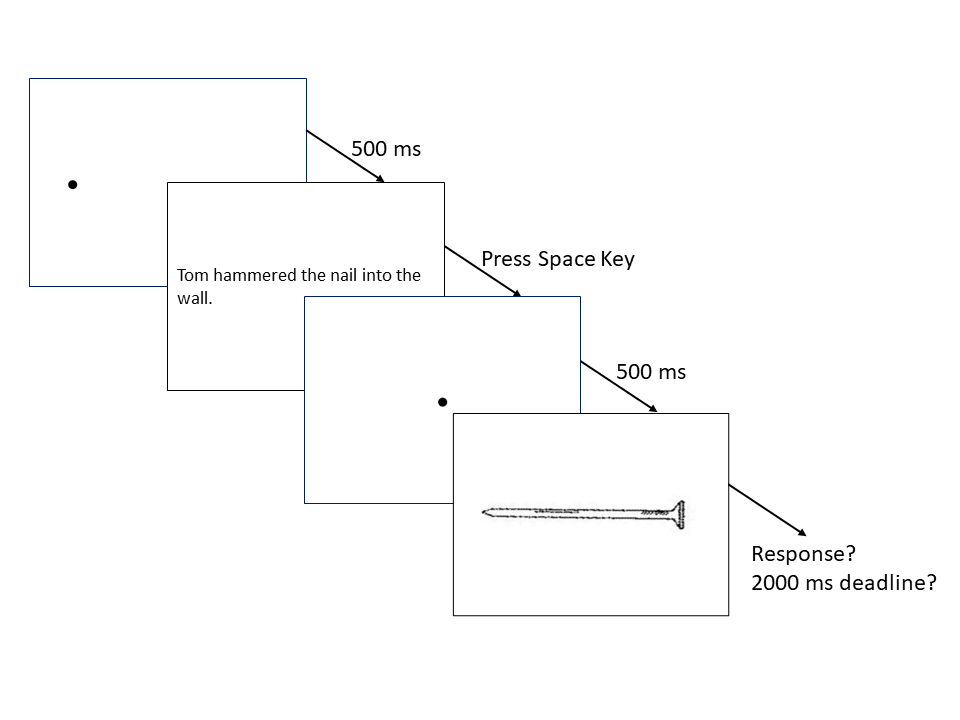
\includegraphics[width=3.2in]{includes/fig/fig2a} \caption{Procedure of sentence-picture verification task.}\label{fig:fig01}
\end{figure}

An additional facet of this research is the linguistic representations of object properties may play a role in the unreliability of the mental simulation effect. Mental simulation effects for object shape have consistently appeared in English (Zwaan et al., 2017; Zwaan \& Madden, 2005; Zwaan \& Pecher, 2012), Chinese (Li \& Shang, 2017), Dutch (De Koning et al., 2017; Engelen et al., 2011; Pecher et al., 2009; Rommers et al., 2013), German (Koster et al., 2018), Croatian (Šetić \& Domijan, 2017), and Japanese (Sato et al., 2013). Object orientation, on the other hand, has produced mixed results across languages (Chen et al., 2020; De Koning et al., 2017; Koster et al., 2018; Zwaan \& Madden, 2005; Zwaan \& Pecher, 2012). Among the studies of shape and orientation, the results indicated smaller effect sizes of object orientation than that of object shape (e.g., d = 0.10 vs.~0.17; in Zwaan and Pecher, 2012; 0.07 vs.~0.27 in de Koning et al., 2017). To understand the causes for the discrepancies among object properties and languages, it is imperative to consider the cross-linguistic and experimental factors of the sentence-picture verification task.

\hypertarget{cross-linguistic-methodological-and-cognitive-factors}{%
\subsection{Cross-linguistic, Methodological, and Cognitive Factors}\label{cross-linguistic-methodological-and-cognitive-factors}}

Several factors might contribute to cross-linguistic differences in the match advantage of orientation, and we focused on context, methodological, and cognitive factors. Researchers have argued that languages differ in how they encode motion and placement events in sentences (Newman, 2002; Verkerk, 2014). In addition, the potential role of mental rotation as a confound has been considered (Rommers et al., 2013). We expand on how the context, experimental, and cognitive factors hinder the improvement of theoretical frameworks as below.

\textbf{Context Factors.} The probe sentences used in object orientation studies usually contain several motion events (e.g., ``The ant walked towards the pot of honey and tried to climb in.''). The languages we probed in this study encode motion events in different ways, and grammatical differences between them could explain the different match advantage results. According to Verkerk (2014), Germanic languages (e.g., Dutch, English, German) generally encode the manner of motion in the verb (e.g., `The ant dashed'), while conveying the path information through satellite adjuncts (e.g., `towards the pot of honey'). In contrast, other languages, such as the Romance family (e.g., Portuguese, Spanish) more often encode path in the verb (e.g., `crossing,' `exiting'). Crucially, the past research on the match advantage of object orientation is exclusively based on Germanic languages, and yet, there were differences across those languages, with English being the only one that consistently yielded the match advantage. As a minor difference across Germanic languages in this regard, Verkerk notes that path-only constructions (e.g., `The ant went to the feast') are more common in English than in other Germanic languages.

Another topic to be considered is the lexical encoding of placement in each language, as the stimuli contains several placement events (e.g., `Sara situated the expensive plate on its holder on the shelf.'). Chen et al. (2020) and Koster et al. (2018) noted that some Germanic languages, such as German and Dutch, often make the orientation of objects more explicit than English. Whereas in English readers could use the verb ``put'' in both ``She put the book on the table'' and ``She put the bottle on the table,'' in both Dutch and German, readers could instead say ``She laid the book on the table,'' and ``She stood the bottle on the table.'' In these literal translations from German and Dutch, the verb ``lay'' encodes a horizontal orientation, whereas the verb ``stand'' encodes a vertical orientation. This distinction extends to verbs indicating existence. As Newman (2002) exemplified, an English speaker would be likely to say ``There's a lamp in the corner,'' whereas a Dutch speaker would be more likely to say ``There `stands' a lamp in the corner.'' Nonetheless, we cannot conclude that these cross-linguistic differences are affecting the match advantage across languages because the current theories (e.g., language and situated simulation, Barsalou, 2008) do not precisely define the complexity of linguistic aspects such as placement events.

\textbf{Methodological factors.} Inconsistent findings on the match advantage of object orientation generated the debates about the reliable task design, such as in the studies failing to detect the match advantage participants not being required to verify the probe sentences they had read (see Zwaan, 2014). Without such a verification, participants might have paid less attention to the meaning of the probe sentences, in which they would have been less likely to form a mental representation of the objects (e.g., Zwaan \& van Oostendorp, 1993). In this regard, it is relevant to acknowledge that variability originating from individual differences and other characteristics of experiments can substantially influence the results (Barsalou, 2019; Kaschak \& Madden, 2021).

\textbf{Cognitive Factors.} Since the first study showed a match advantage of object orientation (Stanfield \& Zwaan, 2001), later studies on this topic have examined the association between the match advantage and alternative cognitive mechanisms rather than the situated simulation. Spatial cognition is one of the potential cognitive mechanisms, which may be measured with mental rotation tasks. Studies have suggested that mental rotation tasks offer valid reflections of previous spatial experience (Frick \& Möhring, 2013) and of current spatial cognition (Chu \& Kita, 2008; Pouw et al., 2014). De Koning et al. (2017) suggested that effectiveness of mental rotation could increase with the object size then facilitate the processing to replace the mismatched orientation described in the sentence. Chen et al. (2020) examined this implication in use of the picture-picture verification task that was designed using the mental rotation paradigm (Cohen \& Kubovy, 1993). In each trial of this task, two pictures appear on opposite sides of the screen. Participants had to verify whether the pictures represent identical or different objects. This study not only indicated the shorter verification times for the same orientation (i.e., two identical pictures presented in horizontal or vertical orientation) but also showed the larger time difference for the large size object (i.e., pictures are bridges versus pictures are pens). The results patterns are consistent among their investigated languages: English, Dutch, and Chinese. In comparison with the results of sentence-picture verification and picture-picture verification, -Chen et al. (2020) revealed the plausible hypothesis that mental rotation may affect the comprehension in some languages whereas in others. This study converted the picture-picture verification times to the mental rotation scores that were the discrepancy of verification times between the identical and different orientation\footnote{In the preregistered plan, we used the term ``imagery score'' but many collaborators hardly realized what the measurement refers to. Therefore, we used ``mental rotation scores'' instead of ``imagery scores'' in the final report.}. With this measurement, we explore the relation of mental rotation in spatial cognition and orientation effect in comprehension across the investigated languages.

\hypertarget{purposes-of-this-study}{%
\subsection{Purposes of this study}\label{purposes-of-this-study}}

To scrutinize the discrepancies of object orientation effects across languages and cognitive factors, we examined the reproducibility of this effect. In this multi-lab collaboration, our preregistered plan aimed at detecting a general match advantage of object orientation across languages and evaluated the magnitude of match advantage in each specific language. Additionally, we examined if match advantages were related to the mental rotation index. Thus, this study followed the original methods from Stanfield and Zwaan (2001) and addressed two primary questions: (1) How much of the match advantage of object orientation can be obtained within different languages and (2) How do differences in the mental rotation index affect the match advantage across languages?

\hypertarget{method}{%
\section{Method}\label{method}}

\hypertarget{hypotheses-and-design}{%
\subsection{Hypotheses and Design}\label{hypotheses-and-design}}

The study design for the sentence-picture and picture-picture verification task was mixed using between-participant (language) and within-participant (match versus mismatch object orientation) independent variables. In the sentence-picture verification task, the match condition reflects a matching between the sentence and the picture, whereas in the picture-picture verification, it reflects a match in orientation between two pictures. The only dependent variable for both tasks was response time. The time difference between conditions in each task are the measurement of orientation effects and mental rotation scores. We did not select languages systematically, but instead based on our collaboration recruitment with the Psychological Science Accelerator (PSA, Moshontz et al., 2018).

\begin{enumerate}
\def\labelenumi{(\arabic{enumi})}
\item
  In the sentence-picture verification task, we expected response time to be shorter for matching compared to mismatching orientations within each language. In the picture-picture verification task, we expected shorter response time for identical orientation compared to different orientations. We did not have any specific hypotheses about the relative size of the object orientation match advantage in different languages.
\item
  Based on the assumption that the mental rotation is a general cognitive aspect, we expect equal mental rotation scores across languages but no association with mental simulation effects (see Chen et al., 2020).
\end{enumerate}

\hypertarget{participants}{%
\subsection{Participants}\label{participants}}

The preregistered power analysis indicated n = 156 to 620 participants for 80\% power for a directional one-sample t-test for a d = 0.20 and 0.10, respectively. A mixed-model simulation suggested that n = 400 participants with 100 items (i.e., 24 planned items nested within at least five languages) would produce 90\% power to detect the same effect as Zwaan and Pecher (2012). The laboratories were allowed to follow a secondary plan: a team collected at least their preregistered minimum sample size (suggested 100 to 160 participants, most implemented 50), and then determine whether or not to continue data collection via Bayesian sequential analysis (stopping data collection if \(BF_{10}\) = 10 or 1/10)\footnote{See details of power analysis in the preregistered plan, p.~13 \textasciitilde{} 15. \url{https://psyarxiv.com/t2pjv/}}.

We finally collected data in 18 languages from 47 laboratories. Each laboratory chose a maximal sample size and an incremental n for sequential analysis before their data collection. Because the preregistered power analysis did not match the final analysis plan, we additionally completed a sensitivity analysis to ensure sample size was adequate to detect small effects, and the results indicated that each effect could be detected at a 2.23 millisecond range for the object orientation effect. Appendix 1 summarizes the details of sensitivity analysis.

Before the pandemic outbreak, 2,340 participants (1,104 women; M = 21.46428 years old) from 29 laboratories joined and finished the study. After the study migrated online, additional 1,403 participants (926 women; M = 21.46428 years old) from 20 laboratories joined this study. Excluded the participants who did not complete the study, 2,007 participants from on-site study and 1,390 participants from online study contributed to the valid data.

In online study participants heard auditory instructions at the beginning and had to correctly answer at least 2 of 3 comprehension check questions about the instructions.
All participating laboratories had either ethical approval or institutional evaluation before data collection. All data and analysis scripts are available on the source files (\url{https://osf.io/p7avr/}). Appendix 2 summarizes the average characteristics by language and laboratory.

\hypertarget{general-procedure-and-materials}{%
\subsection{General Procedure and Materials}\label{general-procedure-and-materials}}

In the beginning of the sentence-picture verification task, participants had to correctly answer all the practice trials. Each trial started with a left-justified and horizontally centered fixation point displayed for 1000 ms, immediately followed by the probe sentence. The sentence was presented until the participant pressed the space key, acknowledging that they understood the sentence. Then, the object picture (from Zwaan \& Pecher, 2012) was presented in the center of the screen until the participant responded otherwise it disappeared after 2 seconds. Participants were instructed to verify that the object on screen was mentioned in the probe sentence as quickly and accurately as they could. Following the original study (Stanfield \& Zwaan, 2001), a memory check test was carried out after every three to eight trials to ensure that the participants had read each sentence carefully.

The picture-picture verification task used the same object pictures. In each trial, two objects appeared on either side of the central fixation point until either the participant indicated that the pictures displayed the same object or two different objects or until 2 seconds elapsed. In the trials where the same object was displayed, the pictures on each side were presented the same orientation (both were horizontal/vertical) or different orientations (one was horizontal; one was vertical).

The study was executed using OpenSesame software for millisecond timing (Mathôt et al., 2012). After the COVID-19 pandemic broke out, the project team decided to move data collection online. To minimize the differences between on-site and web-based studies, we converted the original Python code to Javascript and collected the data using OpenSesame through a JATOS server (Lange et al., 2015). We proceeded with the online study from February to June 2021 after the changes in the procedure were approved by the journal editor and reviewers. Appendix 2 describes the deployment of the scripts and the results of participants' fluency tests. Following the literature, we did not anticipate any theoretically important differences between the two data collection methods (see Anwyl-Irvine et al., 2020; Bridges et al., 2020; de Leeuw \& Motz, 2016). The instructions and experimental scripts are available at the public OSF folder (\url{https://osf.io/e428p/} ``Materials'' in Files).

\hypertarget{analysis-plan}{%
\subsection{Analysis plan}\label{analysis-plan}}

Our first planned analysis\footnote{See the analysis plan in the preregistered plan, p.~19 \textasciitilde{} 20. \url{https://psyarxiv.com/t2pjv/}} employed the fixed-effects meta-analysis model that estimated the match advantage across laboratories and languages. The meta-analysis summarized the median reaction times by match condition then determine the effect size by laboratory. For the languages for which at least two teams collected data, we computed the meta-analytical effect size for these language data.

The planned mixed-effect models used each individual response time as the dependent variable and analyzed the fixed effects of matching condition. The maximal random-effects structure for the models included participant, target item, laboratory, and language\footnote{See the analysis plan in the preregistered plan, p.~21. \url{https://psyarxiv.com/t2pjv/}}. The convergence of random-effects structure were detemined by the comparison of AICs. Because of the data from the Internet after COVID outbreaked, we at first evaluated the mixed-effects model with the fixed effects of match condition and data source and the four random intercepts. This analysis showed no difference between data sources: \emph{b} = 38.90, \emph{SE} = 22.68, \emph{t}( 11.20 ) = 1.72, \emph{p} = 0.11. Therefore, the following mixed-effects models did not separate on-site and the web-based data. Language-specific mixed-effect models were conducted if the meta-analysis showed the positive result.

According to the preregistered analysis plan on the mental rotation scores, we at first evaluated the equality of scores across languages in use of ANOVA. Because the later data collection was on the Internet, we used mixed models instead of ANOVA to evaluate the difference of data sources. The other planned analysis was the linear regression analysis in use of mental rotation scores as the predictor of match advantage.

\textbf{Decision criterion.} \emph{p}-values were interpreted using the preregistered alpha level of .05. \emph{p}-values for each effect were calculated using the Satterthwaite approximation for degrees of freedom (Luke, 2017).

\hypertarget{results}{%
\section{Results}\label{results}}

Among the 3,397 available participants(2,007 onsite; 1,390 online), 96 participants had an accuracy percentage below 70\%. According to the preregistered plan, the analyses excluded these participants' data.\footnote{Low-accurate participants distributed across 27 laboratories. ``ARE\_001'' has 41 participants. ``NZL\_005'' has 8 participants. The other laboratories have 1 \textasciitilde{} 5 participants.}

\hypertarget{intra-lab-analysis-during-data-collection}{%
\subsection{Intra-lab analysis during data collection}\label{intra-lab-analysis-during-data-collection}}

Before data collection, each lab decided whether they wanted to apply a sequential analysis (Schönbrodt et al., 2017) or whether they wanted to settle for a fixed sample size. The preregistered protocol for labs applying sequential analysis established that they could stop data collection upon reaching the preregistered criterion (\(BF_{10} = 10\ or\ -10\)), or the maximal sample size. Each laboratory chose a fixed sample size and an incremental \emph{n} for sequential analysis before their data collection. Two laboratories (HUN 001, TWN 001) stopped data collection at the preregistered criterion, \(BF_{10} = -10\). Fourteen laboratories did not finish the sequential analysis because (1) twelve laboratories were interrupted by the pandemic outbreak; (2) two laboratories (TUR\_007E, TWN\_002E) recruited English-speaking participants for institutional policies. Lab-based records were reported on a public website as each laboratory completed data collection (details are available in Appendix 3).

\hypertarget{inter-lab-analysis-of-final-data}{%
\subsection{Inter-lab analysis of final data}\label{inter-lab-analysis-of-final-data}}

\begin{table}

\caption{\label{tab:summary-languages}Descriptive statistics by language: Total sample size, Average accuracy percentage, Median response times and median absolute deviations (in parentheses) per match condition (Mismatching, Matching); Match advantage (difference in response times).}
\centering
\begin{tabular}[t]{llrrrr}
\toprule
Language & N & Accuracy Percentages & Mismatching & Matching & Match Advantage\\
\midrule
Arabic & 106 & 77 & 525(213.12) & 524(234.62) & 0.75\\
Brazilian Portuguese & 50 & 94 & 637(154.19) & 638(146.04) & -1.75\\
English & 1363 & 93 & 573(132.69) & 570(134.18) & 3.50\\
German & 233 & 125 & 585(100.08) & 568(103.78) & 17.00\\
Greek & 98 & 89 & 748(217.20) & 735(243.89) & 12.75\\
\addlinespace
Hebrew & 146 & 96 & 582(100.82) & 583(114.90) & -0.25\\
Hindi & 79 & 88 & 640(200.15) & 669(241.66) & -29.00\\
Hungarian & 129 & 95 & 626(117.13) & 648(132.69) & -22.00\\
Norwegian & 144 & 96 & 592(126.39) & 608(134.92) & -15.50\\
Polish & 50 & 95 & 597(136.03) & 594(117.87) & 3.25\\
\addlinespace
Portuguese & 60 & 95 & 629(130.84) & 592(131.58) & 36.75\\
Serbian & 130 & 93 & 606(151.97) & 610(160.49) & -4.00\\
Simplified Chinese & 81 & 90 & 702(195.70) & 660(166.05) & 42.00\\
Slovak & 138 & 110 & 620(120.09) & 616(119.35) & 4.00\\
Spanish & 127 & 91 & 668(165.31) & 683(156.41) & -14.50\\
\addlinespace
Thai & 50 & 90 & 664(160.12) & 656(156.41) & 8.75\\
Traditional Chinese & 150 & 93 & 626(133.06) & 618(126.02) & 7.50\\
Turkish & 262 & 109 & 661(157.16) & 640(134.92) & 21.00\\
\bottomrule
\end{tabular}
\end{table}

\textbf{Identification of outliers.} Our preregistered plan included excluding outliers based on a linear mixed-model analysis for participants in the third quantile of the grand intercept (i.e., participants with the longest average response times). Only 49.59 \% of participants' data could pass this criterion. After examining the data from both online and in-person data collection, it became clear that both a minimum response latency and maximum response latency should be employed, as improbable times existed at both ends of the distribution (Kvålseth, 2021; Proctor \& Schneider, 2018). The maximum response latency was calculated as two times the mean absolute deviation plus the median calculated separately for each participant. Two participants' data were excluded becauseif they did not fall between the acceptable minimum (160 ms) and maximum response time range (participant's median response time plus 2 median absolute deviation).

(Insert Table \ref{tab:summary-languages} about here )

\begin{figure}
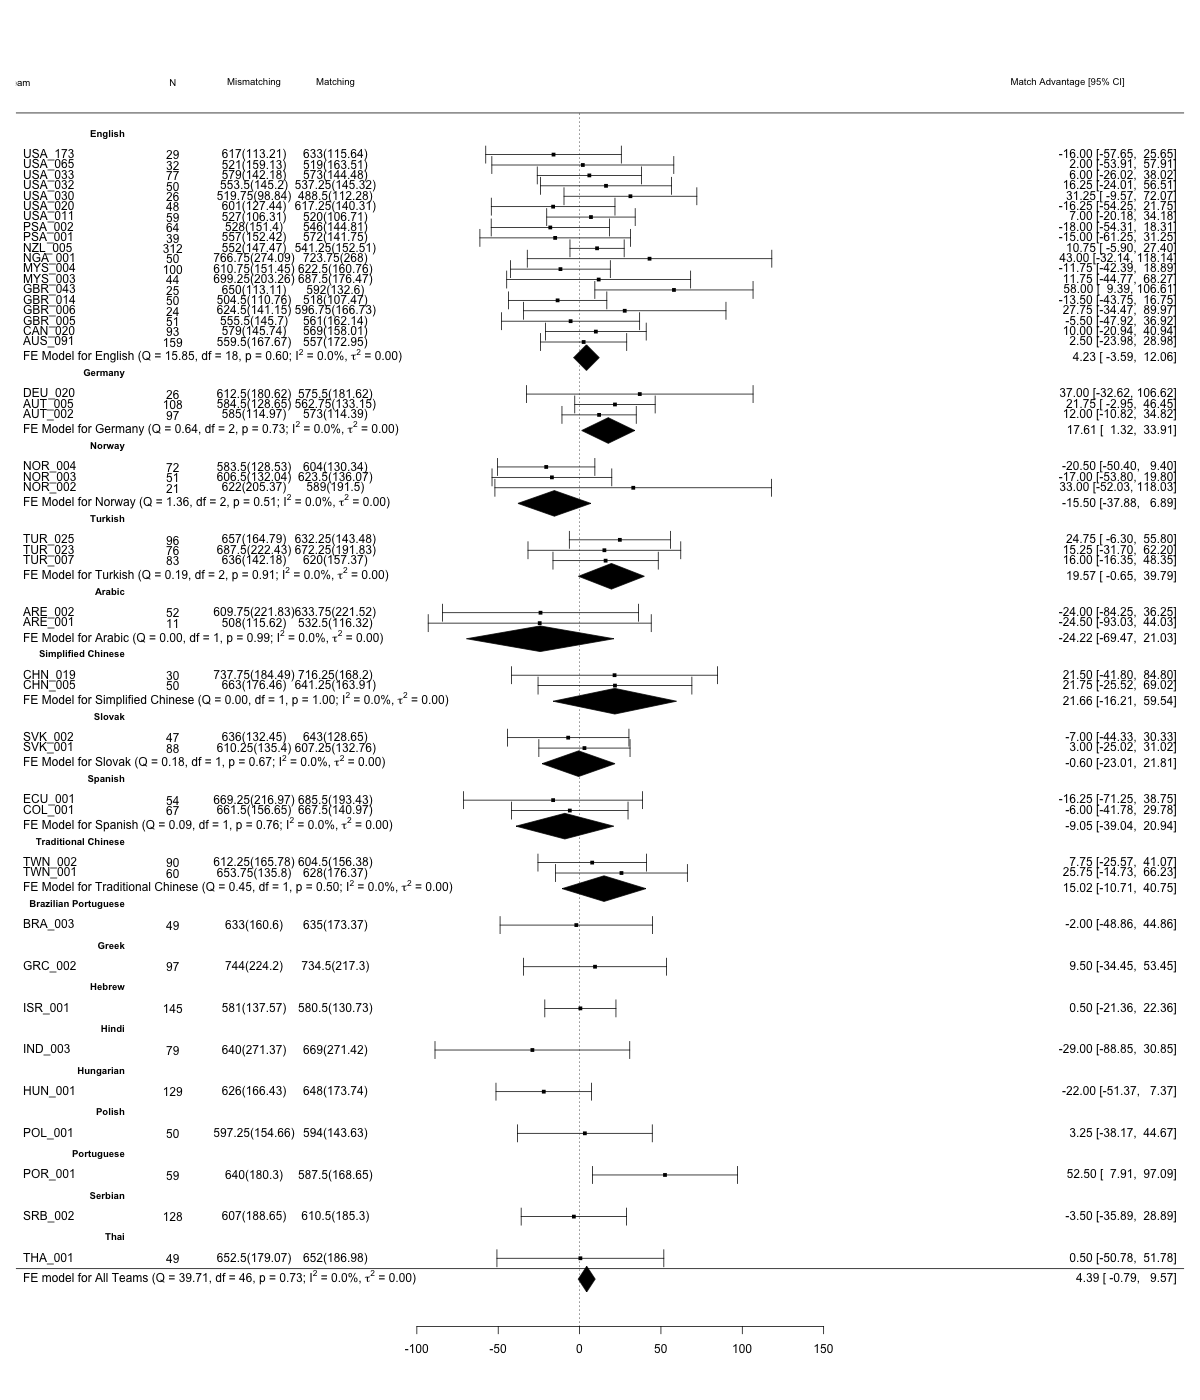
\includegraphics[width=4in]{includes/fig/meta-all} \caption{Meta-analysis on match advantage of object orientation for all languages}\label{fig:meta-all-plot}
\end{figure}

\textbf{Meta-analysis of match advantages across laboratories.} The planned meta-analysis grouped the languages that had at least two laboratories and computed the langage-specific meta-analytic effect (Arabic, English, German, Norway, Simplified Chinese, Traditional Chinese, Slovak, and Turkey). Figure \ref{fig:meta-all-plot} showed a significant meta-analytic effect across German laboratories (\emph{b} = 17.61, 95\% CI {[}1.32, 33.91{]}) and revealed the significant overall effect (\emph{b} = 4.39, 95\% CI {[}-0.79, 9.57{]}).

(Insert Figure \ref{fig:meta-all-plot} about here)

\textbf{Evaluating match advantages using linear mixed-effects models.} As with the analysis plan, the null-effect model of sentence-picture verification data converged at all random intercept factors: participants, items, laboratories, and languages, AIC = 926933.2, BIC = 926988.2; the fixed-effect model either converged at all random intercept factors, AIC = 926932.6, BIC = 926996.9. The fixed-effect model was not significantly different form the null-effect model, \({\chi}^2\) (6,7) = 0.479, \emph{p} = 0.489, and did not reveal a significant effect of match advantage: \emph{b} = 0.771, \emph{SE} = 1.114, t(68049.185) = 0.692, \emph{p} = 0.489. The exploratory analysis evaluated the model with highest theoretical interest that had a random slope of matching condition on language. This model converged at the random intercepts of participants, items, laboratories, and matching conditions on language, AIC = 926935.2, BIC = 927017.8. This model was not significant different from the null-effect model, \({\chi}^2\) (6,9) = 1.853, \emph{p} = 0.604, and showed no significant effect of match advantage: \emph{b} = 1.574, \emph{SE} = 1.218, t(26.837) = 1.293, \emph{p} = 0.207.

We conducted mixed-effect models on German data because this was the only language indicating a significant match advantage in the meta-analysis. The null-effect model converged at the random intercept factors of participants and items but laboratories, AIC = 62667.88, BIC = 62693.96; the fixed-effect model either converged at the random intercept factors of participants and items, AIC = 62662.63, BIC = 62695.22. The fixed-effect model was not significantly different from the null-effect model, \({\chi}^2\) = (4,5) = 3.028, \emph{p} = 0.082, and did not revealed the significant match advantage: \emph{b} = 5.745, \emph{SE} = 3.302, \emph{t}(4733.861) = 1.74, \emph{p} = 0.082. All the details of the above fixed effects and random intercepts are summarized in Appendix 4.

\begin{table}

\caption{\label{tab:lme-coef}Estimated effects and 95\% confidence interval grouped by languages.}
\centering
\begin{tabular}[t]{lrr}
\toprule
Language & Match Advantage & Mental Rotation Score\\
\midrule
Arabic & -10.23 [ -29.22 , 3.72 ] & 23.38 [ 15.74 , 28.99 ]\\
Brazilian Portuguese & -0.03 [ -20.87 , 15.27 ] & 25.22 [ 15.48 , 32.37 ]\\
English & -1.01 [ -4.26 , 1.37 ] & 31.6 [ 29.78 , 32.94 ]\\
German & 5.75 [ -0.73 , 10.5 ] & 30.12 [ 26.32 , 32.92 ]\\
Greek & 10.39 [ -6.16 , 22.55 ] & 28.53 [ 21.36 , 33.79 ]\\
\addlinespace
Hebrew & -3.76 [ -12.6 , 2.74 ] & 27.47 [ 22.6 , 31.05 ]\\
Hindi & -16.62 [ -35.53 , -2.73 ] & 35.68 [ 28.18 , 41.19 ]\\
Hungarian & -4.19 [ -14.92 , 3.68 ] & 25.41 [ 20.19 , 29.25 ]\\
Norwegian & 6.31 [ -3.08 , 13.21 ] & 27.65 [ 22.4 , 31.5 ]\\
Polish & -1.28 [ -17.51 , 10.63 ] & 35.18 [ 27.75 , 40.63 ]\\
\addlinespace
Portuguese & 13.28 [ -2.53 , 24.89 ] & 35.21 [ 26.69 , 41.47 ]\\
Serbian & 2.76 [ -7.83 , 10.54 ] & 27.42 [ 21.77 , 31.56 ]\\
Simplified Chinese & 8.72 [ -6.96 , 20.25 ] & 30.03 [ 22.6 , 35.48 ]\\
Slovak & 2.71 [ -7.64 , 10.32 ] & 32.32 [ 26.95 , 36.27 ]\\
Spanish & 5.07 [ -9 , 15.41 ] & 38.27 [ 30.64 , 43.88 ]\\
\addlinespace
Thai & -2.7 [ -20.58 , 10.43 ] & 31.89 [ 23.97 , 37.71 ]\\
Traditional Chinese & 1.82 [ -8.37 , 9.31 ] & 28.63 [ 23.74 , 32.22 ]\\
Turkish & 2.81 [ -5.85 , 9.17 ] & 36.43 [ 31.78 , 39.84 ]\\
\bottomrule
\end{tabular}
\end{table}

\textbf{Analysis of mental rotation scores.} Followed the analysis plan on the sentence-picture verification data, the analysis on picture-picture verification data at first confirmed the null-effect model converged at all random intercept factors of participants, items, laboratories, and languages, AIC = 877389.4, BIC = 877444.7. To evaluate the affection of data collection sources, we compared the fixed-effect model of data sources and the null-effect model. This fixed-effect model converged at the all random intercept factors, AIC = 877385.5, BIC = 877450, but was not significantly different from the null-effect model, \({\chi}^2\) (6,7) = 0.07, \emph{p} = 0.791.

The planned analysis treated the discrepancy of object orientation settings as the mental rotation scores. The models included the orientation setting as the only one fixed effect converged at all the random intercepts of participants, items, laboratories and orientation setting on languages, AIC = 874667.4, BIC = 874750.3, rather than at the random intercepts of participants, items, laboratories and language, AIC = 874664.9, BIC = 874729.4. There was significant difference between the two models, \({\chi}^2\) (7,9) = 8.174, \emph{p} = 0.017, and the latter model indicated the significant mental rotation scores, \emph{b} = 30.555, \emph{SE} = 1.035, \emph{t}(14.528) = 29.516, \emph{p} \textless{} .001. The coefficients of all considered mixed-effects models are reported in Appendix 5. Table \ref{tab:lme-coef} summarized the language-specific mental rotation scores estimated by the mixed-effect models.

(Insert Table \ref{tab:lme-coef} about here)

\begin{table}

\caption{\label{tab:prediction-coef}Regression coefficient generated from the mental rotation scores. Dependent variable is the match advantages.}
\centering
\begin{tabular}[t]{lrrrrr}
\toprule
Predictor & b & 95\% CI & t & df & p\\
\midrule
Intercept & -6.42 & {}[-23.19, 10.35] & -0.75 & 3366 & .453\\
Brazilian Portuguese & -5.59 & {}[-35.21, 24.03] & -0.37 & 3366 & .711\\
English & 5.58 & {}[-11.84, 22.99] & 0.63 & 3366 & .530\\
German & 13.60 & {}[-6.66, 33.86] & 1.32 & 3366 & .188\\
Greek & 14.50 & {}[-9.70, 38.69] & 1.17 & 3366 & .240\\
\addlinespace
Hebrew & 5.00 & {}[-17.07, 27.06] & 0.44 & 3366 & .657\\
Hindi & -12.30 & {}[-38.06, 13.45] & -0.94 & 3366 & .349\\
Hungarian & -5.06 & {}[-27.70, 17.57] & -0.44 & 3366 & .661\\
Norwegian & 12.07 & {}[-10.09, 34.24] & 1.07 & 3366 & .286\\
Polish & 4.90 & {}[-24.72, 34.52] & 0.32 & 3366 & .746\\
\addlinespace
Portuguese & 19.28 & {}[-8.62, 47.17] & 1.35 & 3366 & .176\\
Serbian & 5.82 & {}[-16.82, 28.46] & 0.50 & 3366 & .614\\
Simplified Chinese & 24.29 & {}[-1.28, 49.86] & 1.86 & 3366 & .063\\
Slovak & 9.44 & {}[-12.89, 31.78] & 0.83 & 3366 & .407\\
Spanish & 5.54 & {}[-17.18, 28.26] & 0.48 & 3366 & .632\\
\addlinespace
Thai & 3.22 & {}[-26.40, 32.84] & 0.21 & 3366 & .831\\
Traditional Chinese & 9.63 & {}[-12.28, 31.54] & 0.86 & 3366 & .389\\
Turkish & 16.93 & {}[-2.97, 36.83] & 1.67 & 3366 & .095\\
\bottomrule
\end{tabular}
\end{table}

\textbf{Prediction model of match advantages.} The last preregistered plan was to build the regression model that could predict the match advantages by the mental rotation scores. If mental rotation scores predicted match advantage, the regression model with languages and mental rotation scores should fit the data better than the regression model with languages only. However, the model comparison indicated the better fitted regression model had languages only, \emph{F} \textless{} 1. As Table \ref{tab:prediction-coef} illustrated, none of the language set of mental rotation scores sufficiently predict the match advantages.

(Insert Table \ref{tab:prediction-coef} about here)

\hypertarget{discussion}{%
\section{Discussion}\label{discussion}}

Measurements on match advantages and mental rotation scores not only revealed the variations of individuals and items but also showed the differences of laboratories and languages. The two planned analysis plans, meta-analysis and mixed-effect models, lead to the divided results. The meta-analysis of match advantages showed the overall orientation effect across the investigated languages, but the language-specific meta-analysis indicated that only German data showed the significant orientation effect. On the other hand, the mixed-effect model did not indicate either the overall effect or the language-specific effect.

Contrary to the match advantages, mixed-effect models indicated significant imagery scores for each investigated language. Regarding the planned regression analysis, it is difficult to the evaluate the predictability of mental rotation scores on the match advantages because of the various results. We summarize the lessons learned on the methodology, analysis, and theoretical issues and attempt to address in which aspect the hypotheses obtained the (dis)confirmative evidence from the current findings.

\hypertarget{methodology-issues}{%
\subsection{Methodology issues}\label{methodology-issues}}

Our data collection deviated from the preregistered plan because 18 of 47 laboratories collected data on the Internet due to the emergence of the Covid-19 pandemic. Because the measurement precision of web-based data is debating (e.g., Anwyl-Irvine et al., 2020; Bridges et al., 2020; de Leeuw \& Motz, 2016), we eventually filtered the outliers in terms of participants' response times instead of the laboratory-based criterion. With the lowest exclusion rate (2.83\%), the fitted mixed-effect model confirmed no difference of response times between on-site and Internet data. Although we mixed the two data sets in the final data analysis, it is worth considering that Internet participants' attention may be easily distracted given the lack of any environmental control and lack of experimenter assistance.

When using sentence-picture verification task as a comprehension task, researchers have had to insert the comprehension questions or memory checks among the experimental trials (Chen et al., 2020; Stanfield \& Zwaan, 2001). Kaschak and Madden (2021) pointed out this setting could trigger the participants to consciously generate mental imagery while reading the probe sentence. If the current results showed significant match advantages, we had to evaluate the contribution of participants' strategy. On the weak positive association of match advantages and mental rotation scores, we could argue that the available strategy to facilitate mental rotation contriubte less to the match advantage. However, it is hardly to indicate that the mental imagery generated from the probe sentences differed from the cognitive processing for mental rotation.

Although the current results were incompatible with past studies (i.e. Chen et al., 2020), the variations among laboratories and languages showed the laboratory practices would decide the results of match (dis)advantages. Beisdes the Internet studies, one of the critical laboratory practices was that participants required explicit hints to comprehend the probe sentences sufficiently. The variation of languages showed the requirements that researchers might design the language-specific hints to trigger the participants' comprehensions.For example, the explict feedbacks of the latest accuracy will promote participants' attention for the coming stimuli.

\hypertarget{analysis-issues}{%
\subsection{Analysis Issues}\label{analysis-issues}}

Although the sensitivity analysis indicated the required number of participants varied among languages, the sources of measurement errors are requiring explorations. One is the limited trials to estimate the orientation effects. From the past to the current studies, the orientation effects were summarized from 24 items (12 match and 12 mismatch). The variation among items could be too large to underestimate the condition means. For example, the orientation effect was 10 ms but the cross-trial variation was 200 ms. In a classical cognitive capacity measurement, such as Stroop task and flanker task, the suggested trial numbers are beyond one-hundred to decrease the trial-level noise (Rouder et al., 2019). In addition to the measurement errors issue, our sensitivity analysis indicated that the massive collaborative study difficulty detected the true effect size in a design of a small number of trials.

This study reflected the difficulty of investigating cognition across languages, especially when dealing with effects that require large sample sizes (see Loken \& Gelman, 2017; Vadillo et al., 2016). In addition to substantial variation in the number of participants available for the investigated languages, the practices to distract the participants' full comprehension of sentence meanings could bias the orientation effects.Twelve languages in this study had one participating team only or did not have sufficient data for the exploratory analysis. On the other hand, the German results indicate that the collected data could reduce the biased estimates among the laboratories. This mass-collaboration model has the benefit to detect the small effect and have a reliable estimation than single-team studies.

\hypertarget{theoretical-issues}{%
\subsection{Theoretical Issues}\label{theoretical-issues}}

Mental simulation theories of comprehension have suggested that cognitive processing converts discourse into either abstract symbols or grounded mental representations (Barsalou, 1999, 2009; Zwaan, 2014). On the other hand, neither theoretical view constituted the priming-based mechanism for the reading task as like sentence-picture verifications. Eventually researchers are unable to improve their understanding on the general language comprehension (Kaschak \& Madden, 2021). Without theoretical guidelines we can not confirm that the orientation effect of German is the product of mental simulations. We also can not accept the null effect in many languages according to the assumption that some language-specific aspects failed to initiate or inhibit the mental simulations. As previously discussed, we learned the measurement errors were from the stimuli content and the secondary task. Without a clear theoretical guideline, researchers hardly specify which physical property robustly facilitate the verification responses and improve the method to precisely measure the mental simulation processing.

The original probe sentences (see Stanfield \& Zwaan, 2001; Zwaan \& Pecher, 2012) were the researchers' creations which were compatible with the experimental demands but did not capture the theoretical complexity. These sentences described the interaction between one actor and one object. The other study (Chen et al., 2020) that found the orientation effect used the researchers' created sentences as well. In comparison with the simple sentences (e.g., Chen et al.~used I saw ``something''), it addressed how the English participants from the original study comprehend the sentences and which language-specific aspects may alter the sentence content in the non-English studies. We suggest the further explorations could employ the original object pictures after simple and complex sentences. The results will help establish specific guidelines for exploring the sentence content.

A secondary task in the sentence-picture verification was used to encourage the participants to understand the probe sentences. In the verification task the participants could make responses without realizing the sentence content. A secondary task asked the probe contents or meanings would require participants to process the sentences. There has been the worry if the secondary task inspired the use of strategies instead of comprehension (e.g., Rommers et al., 2013). This set of studies require the explorations of secondary task demands (memory checks; comprehension questions) and arrangements (fixed trials; flexible trials). These studies are necessary to distinguish the effects from the targeted cognitive processing and strategy in many language topics, such as semantic priming (McNamara, 2005).

\newpage

\hypertarget{references}{%
\section{References}\label{references}}

\begingroup
\setlength{\parindent}{-0.5in}
\setlength{\leftskip}{0.5in}

\hypertarget{refs}{}
\begin{CSLReferences}{1}{0}
\leavevmode\vadjust pre{\hypertarget{ref-anwyl-irvineGorillaOurMidst2020}{}}%
Anwyl-Irvine, A. L., Massonnié, J., Flitton, A., Kirkham, N., \& Evershed, J. K. (2020). Gorilla in our midst: {An} online behavioral experiment builder. \emph{Behavior Research Methods}, \emph{52}(1), 388--407. \url{https://doi.org/10.3758/s13428-019-01237-x}

\leavevmode\vadjust pre{\hypertarget{ref-barsalouEstablishingGeneralizableMechanisms2019}{}}%
Barsalou, L. W. (2019). Establishing generalizable mechanisms. \emph{Psychological Inquiry}, \emph{30}(4), 220--230. \url{https://doi.org/10.1080/1047840X.2019.1693857}

\leavevmode\vadjust pre{\hypertarget{ref-barsalouPerceptualSymbolSystems1999}{}}%
Barsalou, L. W. (1999). Perceptual symbol systems. \emph{Behavioral and Brain Sciences}, \emph{22}, 577--660. \url{https://doi.org/10.1017/S0140525X99002149}

\leavevmode\vadjust pre{\hypertarget{ref-barsalou_grounded_2008}{}}%
Barsalou, L. W. (2008). Grounded cognition. \emph{Annual Review of Psychology}, \emph{59}, 617--645. \url{https://doi.org/10.1146/annurev.psych.59.103006.093639}

\leavevmode\vadjust pre{\hypertarget{ref-barsalouSimulationSituatedConceptualization2009}{}}%
Barsalou, L. W. (2009). Simulation, situated conceptualization, and prediction. \emph{Philosophical Transactions of the Royal Society of London. Series B, Biological Sciences}, \emph{364}, 1281--1289. \url{https://doi.org/10.1098/rstb.2008.0319}

\leavevmode\vadjust pre{\hypertarget{ref-bridgesTimingMegastudyComparing2020a}{}}%
Bridges, D., Pitiot, A., MacAskill, M. R., \& Peirce, J. W. (2020). The timing mega-study: Comparing a range of experiment generators, both lab-based and online. \emph{PeerJ}, \emph{8}, e9414. \url{https://doi.org/10.7717/peerj.9414}

\leavevmode\vadjust pre{\hypertarget{ref-chenDoesObjectSize2020}{}}%
Chen, S.-C., de Koning, B. B., \& Zwaan, R. A. (2020). Does object size matter with regard to the mental simulation of object orientation? \emph{Experimental Psychology}, \emph{67}(1), 56--72. \url{https://doi.org/10.1027/1618-3169/a000468}

\leavevmode\vadjust pre{\hypertarget{ref-chuSpontaneousGesturesMental2008}{}}%
Chu, M., \& Kita, S. (2008). Spontaneous gestures during mental rotation tasks: {Insights} into the microdevelopment of the motor strategy. \emph{Journal of Experimental Psychology: General}, \emph{137}(4), 706--723. \url{https://doi.org/10.1037/a0013157}

\leavevmode\vadjust pre{\hypertarget{ref-cohenMentalRotationMental1993}{}}%
Cohen, D., \& Kubovy, M. (1993). Mental rotation, mental representation, and flat slopes. \emph{Cognitive Psychology}, \emph{25}, 351--382. \url{https://doi.org/10.1006/cogp.1993.1009}

\leavevmode\vadjust pre{\hypertarget{ref-connellRepresentingObjectColour2007}{}}%
Connell, L. (2007). Representing object colour in language comprehension. \emph{Cognition}, \emph{102}, 476--485. \url{https://doi.org/10.1016/j.cognition.2006.02.009}

\leavevmode\vadjust pre{\hypertarget{ref-koning_mental_2017}{}}%
De Koning, B. B., Wassenburg, S. I., Bos, L. T., \& Van der Schoot, M. (2017). Mental simulation of four visual object properties: Similarities and differences as assessed by the sentence-picture verification task. \emph{Journal of Cognitive Psychology}, \emph{29}(4), 420--432. \url{https://doi.org/10.1080/20445911.2017.1281283}

\leavevmode\vadjust pre{\hypertarget{ref-deleeuwPsychophysicsWebBrowser2016}{}}%
de Leeuw, J. R., \& Motz, B. A. (2016). Psychophysics in a {Web} browser? {Comparing} response times collected with {JavaScript} and {Psychophysics Toolbox} in a visual search task. \emph{Behavior Research Methods}, \emph{48}(1), 1--12. \url{https://doi.org/10.3758/s13428-015-0567-2}

\leavevmode\vadjust pre{\hypertarget{ref-engelenPerceptualSimulationDeveloping2011}{}}%
Engelen, J. A. A., Bouwmeester, S., de Bruin, A. B. H., \& Zwaan, R. A. (2011). Perceptual simulation in developing language comprehension. \emph{Journal of Experimental Child Psychology}, \emph{110}(4), 659--675. \url{https://doi.org/10.1016/j.jecp.2011.06.009}

\leavevmode\vadjust pre{\hypertarget{ref-frickMentalObjectRotation2013}{}}%
Frick, A., \& Möhring, W. (2013). Mental object rotation and motor development in 8- and 10-month-old infants. \emph{Journal of Experimental Child Psychology}, \emph{115}(4), 708--720. \url{https://doi.org/10.1016/j.jecp.2013.04.001}

\leavevmode\vadjust pre{\hypertarget{ref-kaschakEmbodimentLabTheory2021}{}}%
Kaschak, M. P., \& Madden, J. (2021). Embodiment in the {Lab}: {Theory}, {Measurement}, and {Reproducibility}. In M. D. Robinson \& L. E. Thomas (Eds.), \emph{Handbook of {Embodied Psychology}} (pp. 619--635). {Springer International Publishing}. \url{https://doi.org/10.1007/978-3-030-78471-3_27}

\leavevmode\vadjust pre{\hypertarget{ref-kosterMentalSimulationObject2018}{}}%
Koster, D., Cadierno, T., \& Chiarandini, M. (2018). Mental simulation of object orientation and size: {A} conceptual replication with second language learners. \emph{Journal of the European Second Language Association}, \emph{2}(1). \url{https://doi.org/10.22599/jesla.39}

\leavevmode\vadjust pre{\hypertarget{ref-kvalsethHickLawEquivalent2021}{}}%
Kvålseth, T. O. (2021). Hick's law equivalent for reaction time to individual stimuli. \emph{British Journal of Mathematical and Statistical Psychology}, \emph{74}(S1), 275--293. \url{https://doi.org/10.1111/bmsp.12232}

\leavevmode\vadjust pre{\hypertarget{ref-langeJustAnotherTool2015}{}}%
Lange, K., Kühn, S., \& Filevich, E. (2015). "{Just Another Tool} for {Online Studies}'' ({JATOS}): {An} easy solution for setup and management of web servers supporting online studies. \emph{PLOS ONE}, \emph{10}(6), e0130834. \url{https://doi.org/10.1371/journal.pone.0130834}

\leavevmode\vadjust pre{\hypertarget{ref-liERPStudyMental2017}{}}%
Li, Y., \& Shang, L. (2017). {An ERP study on the mental simulation of implied object color information during Chinese sentence comprehension}. \emph{Journal of Psychological Science}, \emph{40}(1), 29--36. \url{https://doi.org/10.16719/j.cnki.1671-6981.20170105}

\leavevmode\vadjust pre{\hypertarget{ref-lokenMeasurementErrorReplication2017}{}}%
Loken, E., \& Gelman, A. (2017). Measurement error and the replication crisis. \emph{Science}, \emph{355}(6325), 584--585. \url{https://doi.org/10.1126/science.aal3618}

\leavevmode\vadjust pre{\hypertarget{ref-lukeEvaluatingSignificanceLinear2017}{}}%
Luke, S. G. (2017). Evaluating significance in linear mixed-effects models in {R}. \emph{Behavior Research Methods}, \emph{49}(4), 1494--1502. \url{https://doi.org/10.3758/s13428-016-0809-y}

\leavevmode\vadjust pre{\hypertarget{ref-mathotOpenSesameOpensourceGraphical2012}{}}%
Mathôt, S., Schreij, D., \& Theeuwes, J. (2012). {OpenSesame}: {An} open-source, graphical experiment builder for the social sciences. \emph{Behavior Research Methods}, \emph{44}(2), 314--324. \url{https://doi.org/10.3758/s13428-011-0168-7}

\leavevmode\vadjust pre{\hypertarget{ref-mcnamaraSemanticPrimingPerspectives2005}{}}%
McNamara, T. P. (2005). \emph{Semantic {Priming}: {Perspectives From Memory} and {Word Recognition}}. {Psychology Press}.

\leavevmode\vadjust pre{\hypertarget{ref-moshontzPsychologicalScienceAccelerator2018}{}}%
Moshontz, H., Campbell, L., Ebersole, C. R., IJzerman, H., Urry, H. L., Forscher, P. S., Grahe, J. E., McCarthy, R. J., Musser, E. D., Antfolk, J., Castille, C. M., Evans, T. R., Fiedler, S., Flake, J. K., Forero, D. A., Janssen, S. M. J., Keene, J. R., Protzko, J., Aczel, B., \ldots{} Chartier, C. R. (2018). The {Psychological Science Accelerator}: {Advancing} psychology through a distributed collaborative network. \emph{Advances in Methods and Practices in Psychological Science}, \emph{1}(4), 501--515. \url{https://doi.org/10.1177/2515245918797607}

\leavevmode\vadjust pre{\hypertarget{ref-newmanCrosslinguisticOverviewPosture2002}{}}%
Newman, J. (2002). 1. {A} cross-linguistic overview of the posture verbs {``{Sit},''} {``{Stand},''} and {``{Lie}.''} In J. Newman (Ed.), \emph{Typological {Studies} in {Language}} (Vol. 51, pp. 1--24). {John Benjamins Publishing Company}. \url{https://doi.org/10.1075/tsl.51.02new}

\leavevmode\vadjust pre{\hypertarget{ref-ostarekSixChallengesEmbodiment2019}{}}%
Ostarek, M., \& Huettig, F. (2019). Six {Challenges} for {Embodiment Research}. \emph{Current Directions in Psychological Science}, \emph{28}(6), 593--599. \url{https://doi.org/10.1177/0963721419866441}

\leavevmode\vadjust pre{\hypertarget{ref-pecherLanguageComprehendersRetain2009}{}}%
Pecher, D., van Dantzig, S., Zwaan, R. A., \& Zeelenberg, R. (2009). Language comprehenders retain implied shape and orientation of objects. \emph{The Quarterly Journal of Experimental Psychology}, \emph{62}(6), 1108--1114. \url{https://doi.org/10.1080/17470210802633255}

\leavevmode\vadjust pre{\hypertarget{ref-pouwMoreEmbeddedExtended2014}{}}%
Pouw, W. T. J. L., de Nooijer, J. A., van Gog, T., Zwaan, R. A., \& Paas, F. (2014). Toward a more embedded/extended perspective on the cognitive function of gestures. \emph{Frontiers in Psychology}, \emph{5}. \url{https://doi.org/10.3389/fpsyg.2014.00359}

\leavevmode\vadjust pre{\hypertarget{ref-proctorHickLawChoice2018}{}}%
Proctor, R. W., \& Schneider, D. W. (2018). Hick's law for choice reaction time: {A} review. \emph{Quarterly Journal of Experimental Psychology}, \emph{71}(6), 1281--1299. \url{https://doi.org/10.1080/17470218.2017.1322622}

\leavevmode\vadjust pre{\hypertarget{ref-rommersObjectShapeOrientation2013}{}}%
Rommers, J., Meyer, A. S., \& Huettig, F. (2013). Object shape and orientation do not routinely influence performance during language processing. \emph{Psychological Science}, \emph{24}(11), 2218--2225. \url{https://doi.org/10.1177/0956797613490746}

\leavevmode\vadjust pre{\hypertarget{ref-rouderWhyMostStudies2019}{}}%
Rouder, J., Kumar, A., \& Haaf, J. M. (2019). \emph{Why {Most Studies} of {Individual Differences With Inhibition Tasks Are Bound To Fail}} {[}Preprint{]}. {PsyArXiv}. \url{https://doi.org/10.31234/osf.io/3cjr5}

\leavevmode\vadjust pre{\hypertarget{ref-satoOneWordTime2013}{}}%
Sato, M., Schafer, A. J., \& Bergen, B. K. (2013). One word at a time: {Mental} representations of object shape change incrementally during sentence processing. \emph{Language and Cognition}, \emph{5}(04), 345--373. \url{https://doi.org/10.1515/langcog-2013-0022}

\leavevmode\vadjust pre{\hypertarget{ref-schonbrodtSequentialHypothesisTesting2017}{}}%
Schönbrodt, F. D., Wagenmakers, E.-J., Zehetleitner, M., \& Perugini, M. (2017). Sequential hypothesis testing with {Bayes} factors: {Efficiently} testing mean differences. \emph{Psychological Methods}, \emph{22}(2), 322--339. \url{https://doi.org/10.1037/met0000061}

\leavevmode\vadjust pre{\hypertarget{ref-scorolli2014embodiment}{}}%
Scorolli, C. (2014). Embodiment and language. In L. Shapiro (Ed.), \emph{The {Routledge} handbook of embodied cognition} (pp. 145--156). {Routledge}.

\leavevmode\vadjust pre{\hypertarget{ref-seticNumericalCongruencyEffect2017}{}}%
Šetić, M., \& Domijan, D. (2017). Numerical {Congruency Effect} in the {Sentence-Picture Verification Task}. \emph{Experimental Psychology}, \emph{64}(3), 159--169. \url{https://doi.org/10.1027/1618-3169/a000358}

\leavevmode\vadjust pre{\hypertarget{ref-stanfield_effect_2001}{}}%
Stanfield, R. A., \& Zwaan, R. A. (2001). The effect of implied orientation derived from verbal context on picture recognition. \emph{Psychological Science}, \emph{12}(2), 153--156. \url{https://doi.org/10.1111/1467-9280.00326}

\leavevmode\vadjust pre{\hypertarget{ref-vadilloUnderpoweredSamplesFalse2016}{}}%
Vadillo, M. A., Konstantinidis, E., \& Shanks, D. R. (2016). Underpowered samples, false negatives, and unconscious learning. \emph{Psychonomic Bulletin \& Review}, \emph{23}(1), 87--102. \url{https://doi.org/10.3758/s13423-015-0892-6}

\leavevmode\vadjust pre{\hypertarget{ref-verkerkEvolutionaryDynamicsMotion2014}{}}%
Verkerk, A. (2014). \emph{The evolutionary dynamics of motion event encoding.} {[}PhD thesis{]}. Radboud Universiteit Nijmegen.

\leavevmode\vadjust pre{\hypertarget{ref-zwaan_embodiment_2014}{}}%
Zwaan, R. A. (2014). Embodiment and language comprehension: Reframing the discussion. \emph{Trends in Cognitive Sciences}, \emph{18}(5), 229--234. \url{https://doi.org/10.1016/j.tics.2014.02.008}

\leavevmode\vadjust pre{\hypertarget{ref-zwaanParticipantNonnaiveteReproducibility2017}{}}%
Zwaan, R. A., Diane Pecher, Paolacci, G., Bouwmeester, S., Verkoeijen, P., Dijkstra, K., \& Zeelenberg, R. (2017). Participant {Nonnaiveté} and the reproducibility of cognitive psychology. \emph{Psychonomic Bulletin \& Review}, 1--5. \url{https://doi.org/10.3758/s13423-017-1348-y}

\leavevmode\vadjust pre{\hypertarget{ref-zwaanEmbodiedSentenceComprehension2005}{}}%
Zwaan, R. A., \& Madden, C. J. (2005). Embodied sentence comprehension. In D. Pecher \& R. A. Zwaan (Eds.), \emph{Grounding cognition: {The} role of perception and action in memory, language, and thinking} (pp. 224--245). {Cambridge University Press}.

\leavevmode\vadjust pre{\hypertarget{ref-zwaanRevisitingMentalSimulation2012}{}}%
Zwaan, R. A., \& Pecher, D. (2012). Revisiting mental simulation in language comprehension: Six replication attempts. \emph{PLoS ONE}, \emph{7}, e51382. \url{https://doi.org/10.1371/journal.pone.0051382}

\leavevmode\vadjust pre{\hypertarget{ref-zwaanLanguageComprehendersMentally2002}{}}%
Zwaan, R. A., Stanfield, R. A., \& Yaxley, R. H. (2002). Language comprehenders mentally represent the shapes of objects. \emph{Psychological Science}, \emph{13}, 168--171. \url{https://doi.org/10.1111/1467-9280.00430}

\leavevmode\vadjust pre{\hypertarget{ref-zwaanReadersConstructSpatial1993}{}}%
Zwaan, R. A., \& van Oostendorp, H. (1993). Do readers construct spatial representations in naturalistic story comprehension? \emph{Discourse Processes}, \emph{16}(1-2), 125--143. \url{https://doi.org/10.1080/01638539309544832}

\end{CSLReferences}

\endgroup


\end{document}
